\documentclass[pdftex,12pt]{article}\usepackage[]{graphicx}\usepackage[]{color}
%% maxwidth is the original width if it is less than linewidth
%% otherwise use linewidth (to make sure the graphics do not exceed the margin)
\makeatletter
\def\maxwidth{ %
  \ifdim\Gin@nat@width>\linewidth
    \linewidth
  \else
    \Gin@nat@width
  \fi
}
\makeatother

\definecolor{fgcolor}{rgb}{0.345, 0.345, 0.345}
\newcommand{\hlnum}[1]{\textcolor[rgb]{0.686,0.059,0.569}{#1}}%
\newcommand{\hlstr}[1]{\textcolor[rgb]{0.192,0.494,0.8}{#1}}%
\newcommand{\hlcom}[1]{\textcolor[rgb]{0.678,0.584,0.686}{\textit{#1}}}%
\newcommand{\hlopt}[1]{\textcolor[rgb]{0,0,0}{#1}}%
\newcommand{\hlstd}[1]{\textcolor[rgb]{0.345,0.345,0.345}{#1}}%
\newcommand{\hlkwa}[1]{\textcolor[rgb]{0.161,0.373,0.58}{\textbf{#1}}}%
\newcommand{\hlkwb}[1]{\textcolor[rgb]{0.69,0.353,0.396}{#1}}%
\newcommand{\hlkwc}[1]{\textcolor[rgb]{0.333,0.667,0.333}{#1}}%
\newcommand{\hlkwd}[1]{\textcolor[rgb]{0.737,0.353,0.396}{\textbf{#1}}}%

\usepackage{framed}
\makeatletter
\newenvironment{kframe}{%
 \def\at@end@of@kframe{}%
 \ifinner\ifhmode%
  \def\at@end@of@kframe{\end{minipage}}%
  \begin{minipage}{\columnwidth}%
 \fi\fi%
 \def\FrameCommand##1{\hskip\@totalleftmargin \hskip-\fboxsep
 \colorbox{shadecolor}{##1}\hskip-\fboxsep
     % There is no \\@totalrightmargin, so:
     \hskip-\linewidth \hskip-\@totalleftmargin \hskip\columnwidth}%
 \MakeFramed {\advance\hsize-\width
   \@totalleftmargin\z@ \linewidth\hsize
   \@setminipage}}%
 {\par\unskip\endMakeFramed%
 \at@end@of@kframe}
\makeatother

\definecolor{shadecolor}{rgb}{.97, .97, .97}
\definecolor{messagecolor}{rgb}{0, 0, 0}
\definecolor{warningcolor}{rgb}{1, 0, 1}
\definecolor{errorcolor}{rgb}{1, 0, 0}
\newenvironment{knitrout}{}{} % an empty environment to be redefined in TeX

\usepackage{alltt}
\usepackage[T2A]{fontenc}
\usepackage[utf8]{inputenc}
\usepackage[russian,british]{babel}
\usepackage{csquotes}

\usepackage[paper=a4paper,top=15mm, bottom=15mm,left=15mm,right=10mm,includefoot]{geometry}
\usepackage[pdftex,unicode,colorlinks=true,urlcolor=blue,hyperindex,breaklinks]{hyperref} 

\usepackage{color}
\usepackage{floatflt}
\usepackage{float}
\usepackage{graphicx}
\usepackage{fancyhdr}
\usepackage{booktabs}
\usepackage{longtable}
\usepackage{setspace}
\usepackage{multirow} 
\usepackage{eurosym}
\usepackage{verbatim}
\usepackage{dcolumn}
\usepackage{amsmath}
\usepackage{amsfonts}
\usepackage{amssymb}
%\usepackage{hyperref}
\usepackage{indentfirst} % indent first line
\usepackage{caption}
\newcommand{\e}{\varepsilon}
\usepackage{chngpage}
\usepackage{lscape}
\def\baselinestretch{3}
\IfFileExists{upquote.sty}{\usepackage{upquote}}{}
\begin{document}

$\ln y_i = \beta_1 + \beta_2 \ln l_i + \beta_3 \ln k_i + \e_i$

$T = \frac{(RSS_{R} - RSS_{UR})/q}{RSS_{UR}/(n - k)}$

$R^2 = \frac{ESS}{TSS} = \frac{\hat{\beta}_2^2 \textbf{x}^T \textbf{x}^{(2)}}{\textbf{y}^T \textbf{y}} = \frac{\textbf{x}^T \textbf{y}^{(2)}}{(\textbf{x}^T \textbf{x})(\textbf{y}^T \textbf{y})} = \mathrm{Corr}^2(X, Y)$

\def\baselinestretch{1.5}





\begin{knitrout}
\definecolor{shadecolor}{rgb}{0.969, 0.969, 0.969}\color{fgcolor}\begin{kframe}
\begin{alltt}
\hlkwd{library}\hlstd{(}\hlstr{"dplyr"}\hlstd{)}
\hlstd{data} \hlkwb{<-} \hlkwd{read.csv}\hlstd{(}\hlstr{"data.csv"}\hlstd{,} \hlkwc{header}\hlstd{=}\hlnum{TRUE}\hlstd{)}
\hlkwd{summary}\hlstd{(data)}
\end{alltt}
\end{kframe}
\end{knitrout}


\begin{knitrout}
\definecolor{shadecolor}{rgb}{0.969, 0.969, 0.969}\color{fgcolor}\begin{kframe}
\begin{alltt}
\hlstd{str_stand} \hlkwb{<-} \hlkwa{function}\hlstd{(}\hlkwc{z}\hlstd{) \{}
  \hlstd{z} \hlopt \hlkwd{tolower}\hlstd{()} \hlopt \hlkwd{str_trim}\hlstd{()} \hlopt
    \hlkwd{stri_trans_general}\hlstd{(}\hlkwc{id} \hlstd{=} \hlstr{"Russian-Latin/BGN"} \hlstd{)} \hlopt
    \hlkwd{str_replace_all}\hlstd{(}\hlstr{"[[:punct:]]"}\hlstd{,}\hlstr{" "}\hlstd{)} \hlopt
    \hlkwd{str_replace_all}\hlstd{(}\hlstr{" +"}\hlstd{,}\hlstr{" "}\hlstd{)} \hlopt \hlkwd{return}\hlstd{()}
\hlstd{\}}
\end{alltt}
\end{kframe}
\end{knitrout}


\begin{knitrout}
\definecolor{shadecolor}{rgb}{0.969, 0.969, 0.969}\color{fgcolor}\begin{kframe}
\begin{alltt}
\hlstd{ct.add} \hlkwb{<-} \hlkwd{left_join}\hlstd{(d,ct)} \hlopt
  \hlkwd{mutate}\hlstd{(}\hlkwc{dist}\hlstd{=}\hlkwd{stringdist}\hlstd{(}\hlkwd{str_stand}\hlstd{(user_ans),in_cat))} \hlopt
  \hlkwd{filter}\hlstd{(dist}\hlopt{<}\hlnum{4}\hlstd{)} \hlopt
  \hlkwd{select}\hlstd{(}\hlkwc{in_cat}\hlstd{=user_ans,out_cat)} \hlopt
  \hlkwd{unique}\hlstd{()}
\end{alltt}
\end{kframe}
\end{knitrout}




\begin{knitrout}
\definecolor{shadecolor}{rgb}{0.969, 0.969, 0.969}\color{fgcolor}
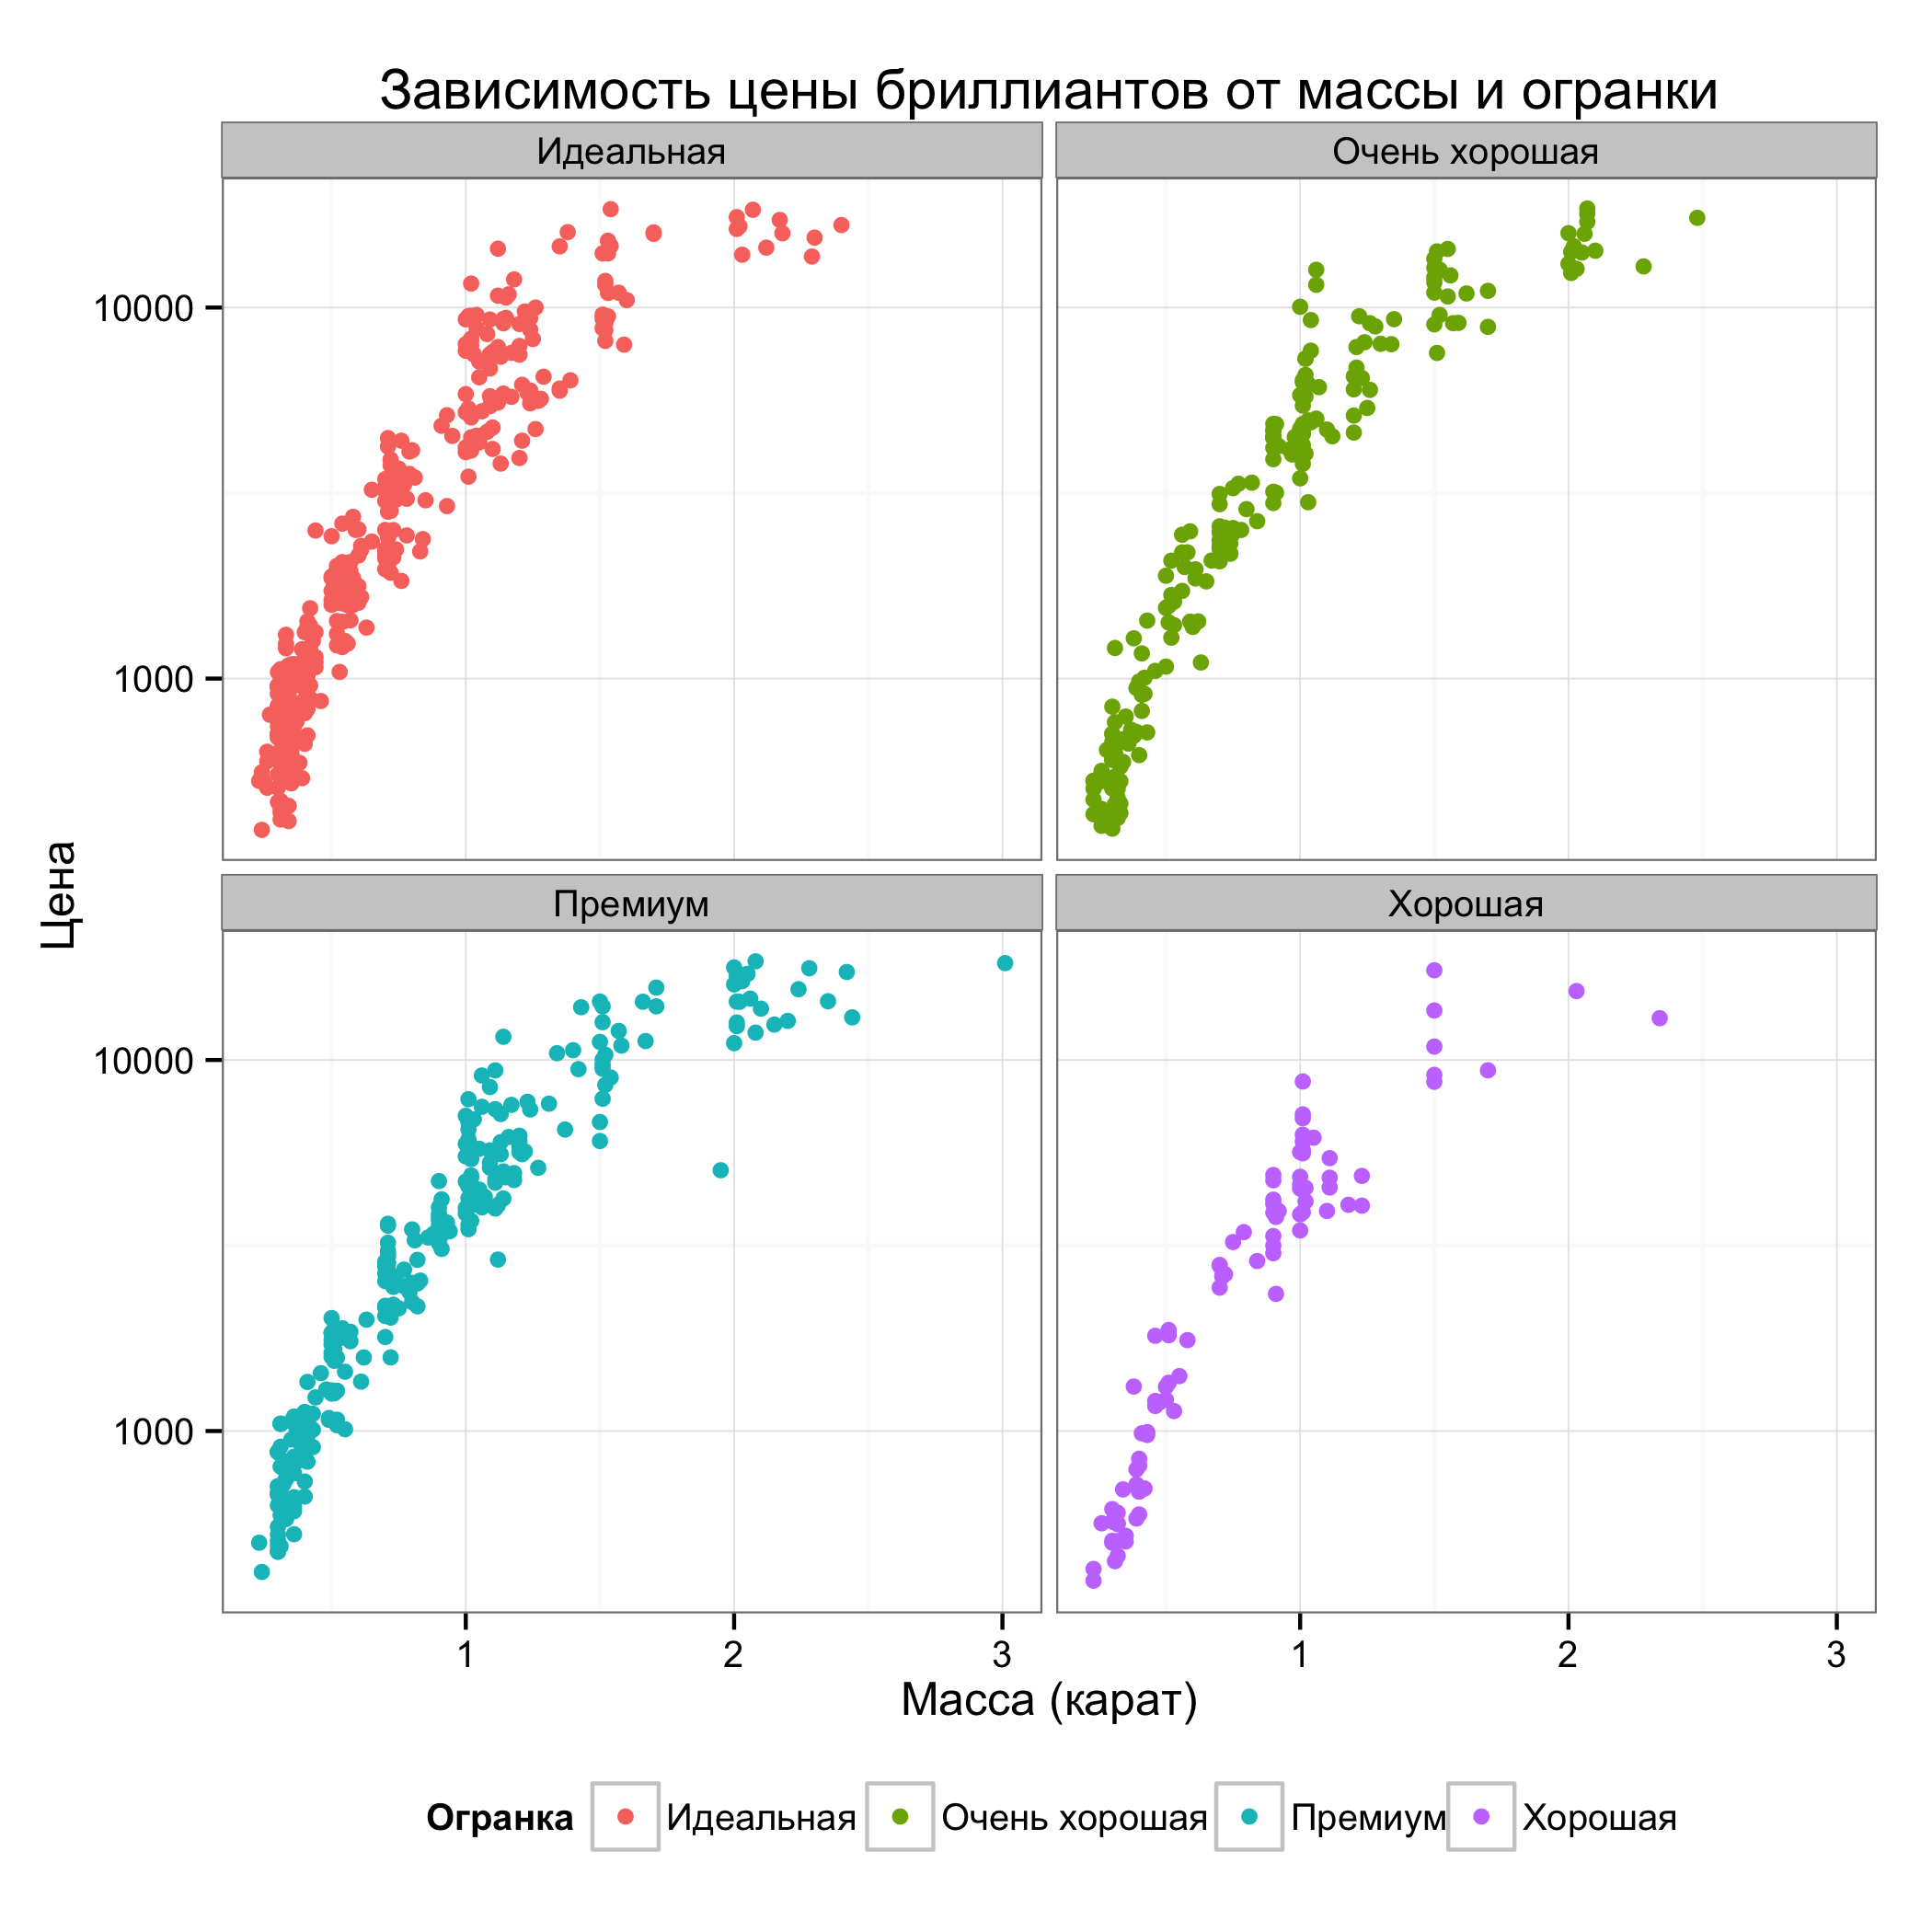
\includegraphics[width=15cm,height=15cm]{figure/unnamed-chunk-6} 

\end{knitrout}

\begin{knitrout}
\definecolor{shadecolor}{rgb}{0.969, 0.969, 0.969}\color{fgcolor}
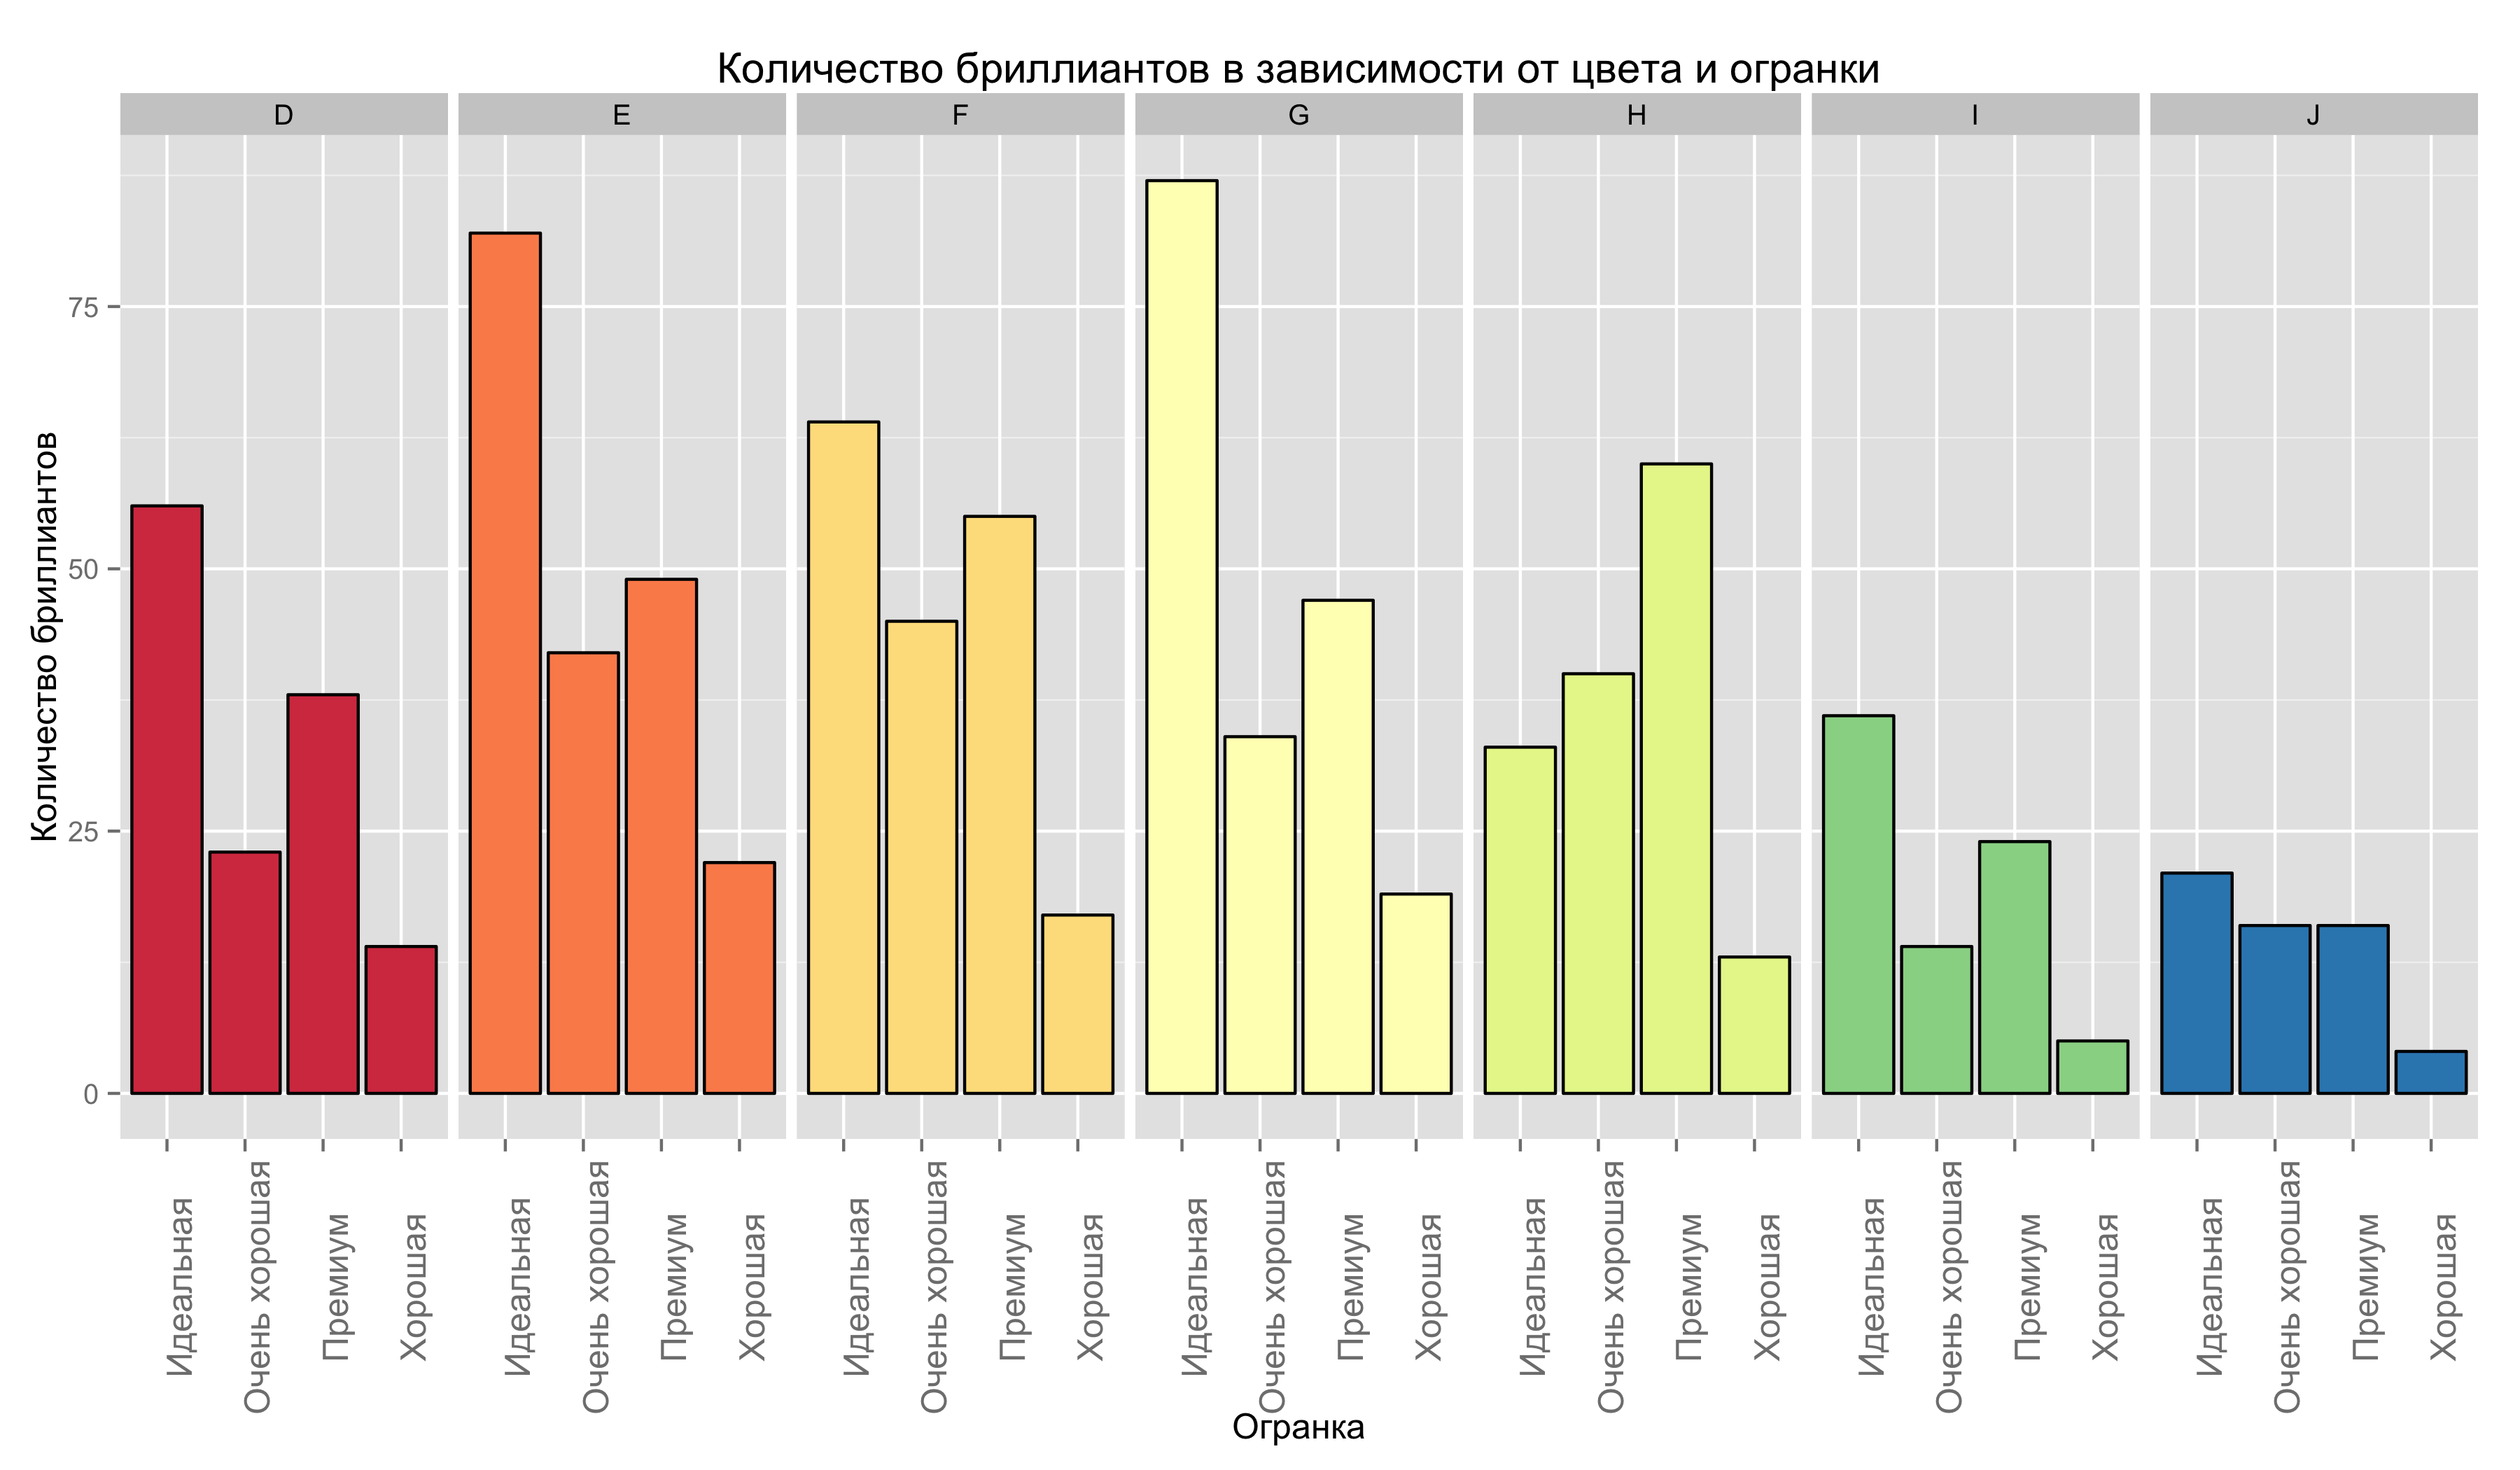
\includegraphics[width=\maxwidth]{figure/unnamed-chunk-7} 

\end{knitrout}

\newpage
\begin{center}
Характеристики российских дефолтных компаний среднего и малого бизнеса
\vspace{0.3cm}
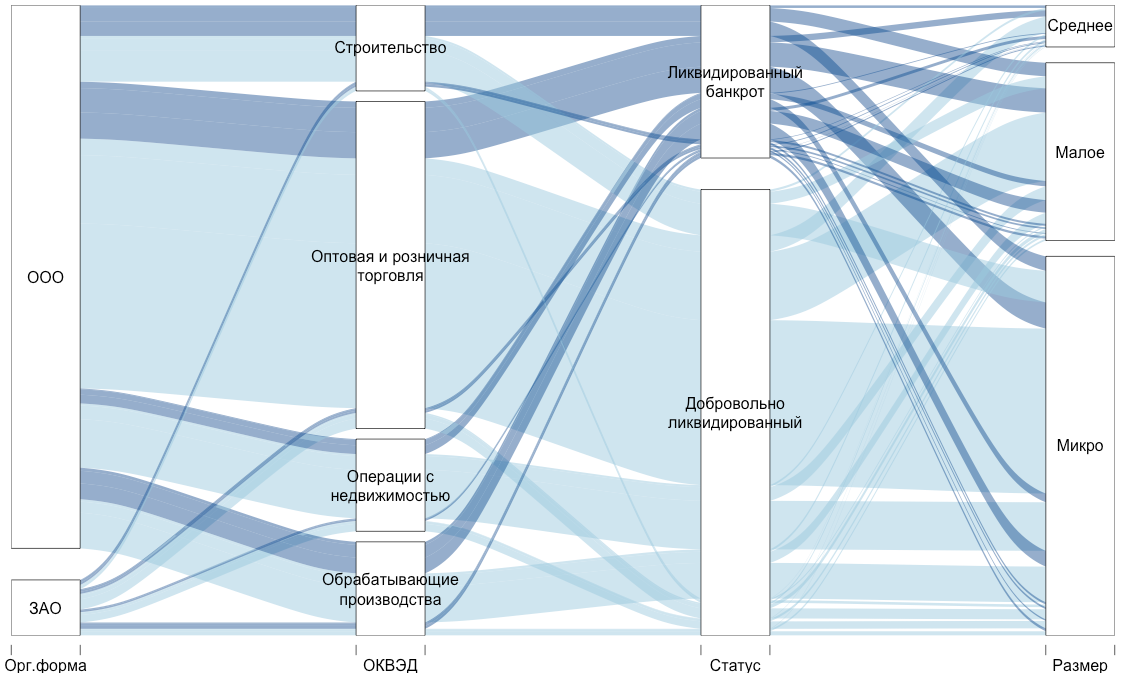
\includegraphics[width=17cm,height=11.5cm]{plot1a.jpeg}

\end{center}

\end{document}
